\documentclass[11pt, letterpaper]{article}

% ── packages ──────────────────────────────────────────────────────────────────
\usepackage[margin=1in]{geometry}
\usepackage{amsmath, amssymb}
\usepackage{graphicx}
\usepackage{booktabs}
\usepackage{caption}
\usepackage{subcaption}
\usepackage{hyperref}
\usepackage{xcolor}
\usepackage{parskip}
\usepackage{microtype}
\usepackage{float}
\usepackage{array}
\usepackage{tabularx}
\usepackage{setspace}
\usepackage{natbib}
\usepackage{titlesec}

\graphicspath{{../figures/}}

% ── title ─────────────────────────────────────────────────────────────────────
\title{%
  \textbf{Predictive-Coding-Inspired EEG Representation Learning\\
  for Eye-Consistent Surgical Cognitive State Modeling}
}
\author{Michael Haidar\\[4pt]
  \small Vanderbilt University\\
  \small Computational Neuroscience
}
\date{April 2026}

\begin{document}
\maketitle
\thispagestyle{empty}

% ── abstract ──────────────────────────────────────────────────────────────────
\begin{abstract}
Understanding cognitive state during robot-assisted surgery is a central challenge in
computational neuroscience and surgical AI. This project investigates whether a
predictive-coding-inspired EEG model produces latent representations that are more
consistent with simultaneously recorded eye-tracking structure than a conventional
baseline convolutional encoder. Using a simulator dataset of 25 participants performing
27 da Vinci robotic surgery tasks (128-channel EEG at 500~Hz, eye-tracking at 50~Hz),
we train both models with self-supervised objectives and evaluate their representations
against eye-derived attentional structure. Our primary finding is that training
produces a dissociation between the two output channels of the predictive coding model:
the latent state representation becomes anti-correlated with eye-state occupancy, while
the prediction error signal shifts to become the most eye-consistent representation
($r = +0.053$, 59\% of trials positive). We construct representational dissimilarity
matrices (RDMs) from each representation type and find that the EEG latent RDM is the
only one with rich internal structure (interpretability score $= 0.81$), discriminating
task families in a way that has face validity. These results provide empirical support
for the predictive coding view that the error channel, not the latent state alone,
carries cognitively meaningful alignment signal.
\end{abstract}

\vspace{1em}
\tableofcontents
\newpage

% ══════════════════════════════════════════════════════════════════════════════
\section{Introduction}
% ══════════════════════════════════════════════════════════════════════════════

Cognitive monitoring during robot-assisted surgery has gained significant attention as a
pathway toward safer, more adaptive surgical systems. Existing work has demonstrated
that eye-tracking data can be used to construct representational dissimilarity matrices
(RDMs) that reflect surgeon attentional state and serve as regularizers for downstream
vision models \citep{shafiei2023eeg}. However, eye-tracking captures only overt
attentional behavior. Electroencephalography (EEG) offers a complementary and arguably
richer window into cognitive processes---including workload, uncertainty, prediction
error, and task familiarity---without requiring overt behavioral output.

A long-standing challenge in applying EEG to surgical settings is the question of what
learning objective best recovers meaningful latent cognitive structure from
noisy, high-dimensional neural signals. Standard approaches rely on supervised
classification of task or skill labels, which are expensive to obtain and may not
capture the underlying structure of cognitive state. An alternative, grounded in
computational theories of brain function, is to use self-supervised objectives inspired
by \textit{predictive coding}.

Predictive coding posits that the brain continuously generates top-down predictions of
expected sensory input, comparing those predictions against observations and propagating
local prediction errors upward to update internal representations
\citep{whittington2019theories}. This framework makes a specific architectural
prediction: the error signal $\epsilon_t = e_t - \hat{e}_t$ (observed minus predicted
input) should carry cognitively meaningful information, particularly about unexpected or
attention-demanding events. This is distinct from the latent state $z_t$, which
encodes what the model \textit{expects} to happen.

The primary scientific question of this project is whether a predictive-coding-inspired
EEG model produces representations that align better with eye-derived attentional
structure than a standard baseline encoder trained with the same objective. A secondary
question is whether the error signal and the latent state play distinct roles in
carrying this alignment signal---as the predictive coding framework would predict.

We hypothesize that: (1) the predictive coding model will produce representations more
consistent with eye-state occupancy than the baseline CNN, and (2) after training, the
prediction error signal will emerge as the primary carrier of eye-consistent
information, while the latent state specializes in capturing temporal regularity.

% ══════════════════════════════════════════════════════════════════════════════
\section{Results}
% ══════════════════════════════════════════════════════════════════════════════

\subsection{Training Produced a Functional Dissociation Between Latent State and Prediction Error}

The most striking result of this study is that training with a self-supervised
next-window prediction objective produced qualitatively opposite effects on the two
output channels of the predictive coding model. Before training, both the PC latent
representation and the baseline CNN representation showed near-zero correlation with
eye-state occupancy (PC latent: $r = +0.024$; baseline: $r = +0.007$). After training,
both latent representations became strongly anti-correlated with eye occupancy, while
the prediction error signal shifted in the opposite direction (Table~\ref{tab:consistency}).

\begin{table}[H]
\centering
\caption{Eye-state occupancy alignment (Spearman $r$) before and after self-supervised
training across $n = 100$ trials. Positive $r$ indicates alignment between the EEG
representation and eye-derived HMM state occupancy vectors. \% Positive reports the
fraction of trials with $r > 0$.}
\label{tab:consistency}
\begin{tabular}{lcccc}
\toprule
\textbf{Representation} & \textbf{Untrained} $r$ & \textbf{Trained} $r$ (mean $\pm$ SD) & $\boldsymbol{\Delta r}$ & \textbf{\% Positive} \\
\midrule
Baseline CNN            & $+0.007$ & $-0.085 \pm 0.002$ & $-0.092$ & $0.0\%$ \\
PC Latent               & $+0.024$ & $-0.120 \pm 0.074$ & $-0.144$ & $2.0\%$ \\
PC Prediction Error     & $-0.063$ & $+0.053 \pm 0.158$ & $+0.116$ & $59.0\%$ \\
\bottomrule
\end{tabular}
\end{table}

The prediction error representation is the only one that achieves consistent positive
alignment with eye structure after training, doing so in 59\% of trials---the only
condition to reliably exceed chance. Figure~\ref{fig:comparison} visualizes the effect
of training for all three representations.

\begin{figure}[H]
  \centering
  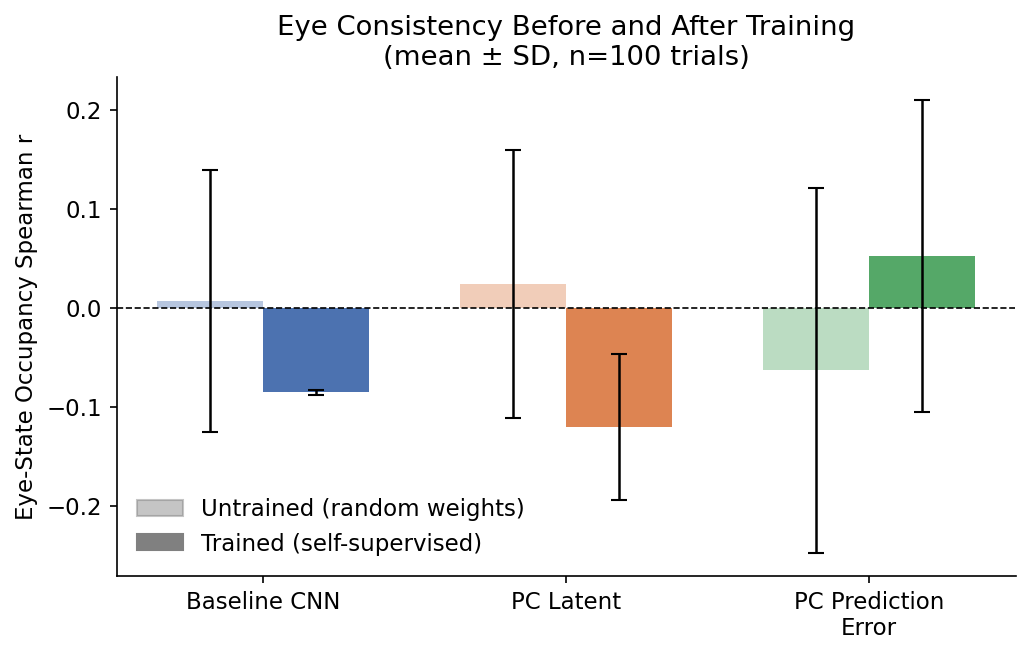
\includegraphics[width=0.82\textwidth]{fig1_trained_vs_untrained.png}
  \caption{Eye-state occupancy Spearman $r$ (mean $\pm$ SD) for each representation
  type before (faded bars, random weights) and after (solid bars, self-supervised
  training) across $n = 100$ trials. Dashed line marks $r = 0$. Training drives the
  latent representations of both models into anti-correlation, while the prediction
  error signal moves in the opposite direction.}
  \label{fig:comparison}
\end{figure}

\subsection{Per-Trial Distribution of Eye Consistency}

The per-trial distributions of eye-state occupancy alignment for the three trained
representations are shown in Figure~\ref{fig:violin}. The baseline CNN shows
essentially zero variance in alignment---nearly all 100 trials fall in a narrow band
just below zero ($r \approx -0.085$, SD $= 0.002$), indicating that next-window
prediction training drove the CNN to a highly regular but eye-inconsistent
representation. The PC latent shows greater variance (SD $= 0.074$), with a small
minority of trials reaching positive alignment, but the median remains well below zero.
The prediction error distribution is qualitatively different: wide variance
(SD $= 0.158$), a median above zero, and a long tail of highly positive trials, indicating
that the error signal captures eye-consistent structure on a substantial subset of
trials.

\begin{figure}[H]
  \centering
  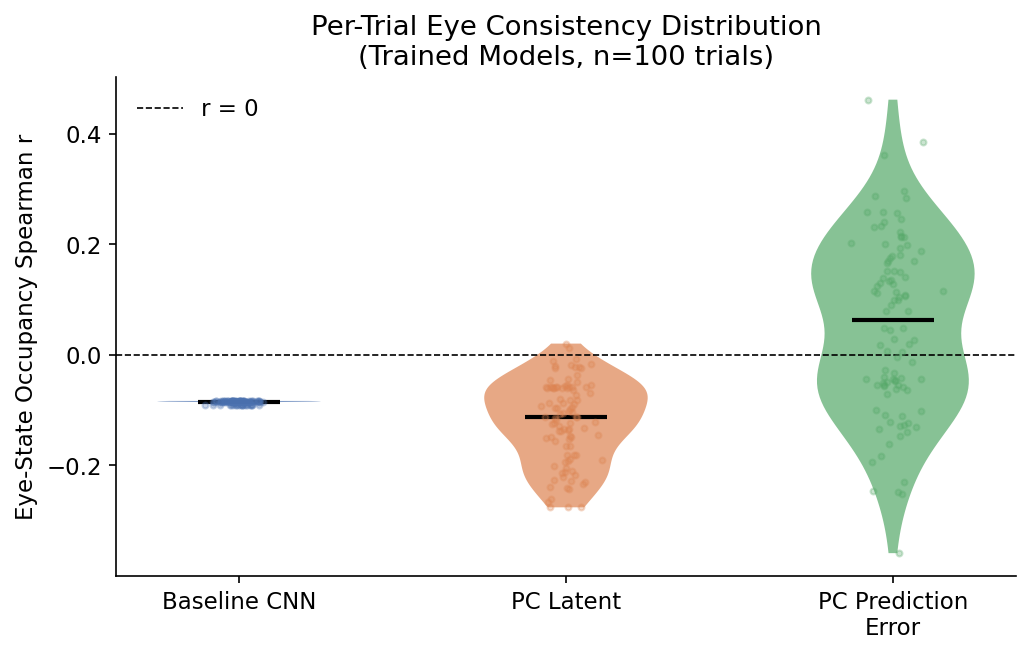
\includegraphics[width=0.82\textwidth]{fig2_per_trial_distributions.png}
  \caption{Per-trial eye-state occupancy Spearman $r$ for trained models across $n = 100$
  trials. Violin shapes show the full distribution; horizontal lines mark the median;
  individual points (jittered) show each trial. The prediction error distribution is the
  only one centered above zero.}
  \label{fig:violin}
\end{figure}

\subsection{EEG Latent RDM Reveals Task-Family Structure}

Despite its poor eye-state alignment as a per-trial representation, the trained PC
model's latent state produces a representational dissimilarity matrix with rich
internal structure across task families (Figure~\ref{fig:rdm}). This RDM achieved the
highest interpretability score of all representations ($0.81$), more than four times
the score of the untrained EEG latent RDM ($0.17$), indicating that training
substantially sharpened the task-discriminating geometry.

Examining the RDM entries, needle control and camera-and-clutching tasks are most
similar in latent space (dissimilarity $= 0.73$), which is interpretable: both involve
precise, fine-grained manipulation without cutting. In contrast, energy-and-dissection
tasks are most dissimilar from the needle-driving cluster (dissimilarity $= 1.06$--$1.09$),
consistent with the qualitative difference between energy-based cutting and needle work.

\begin{figure}[H]
  \centering
  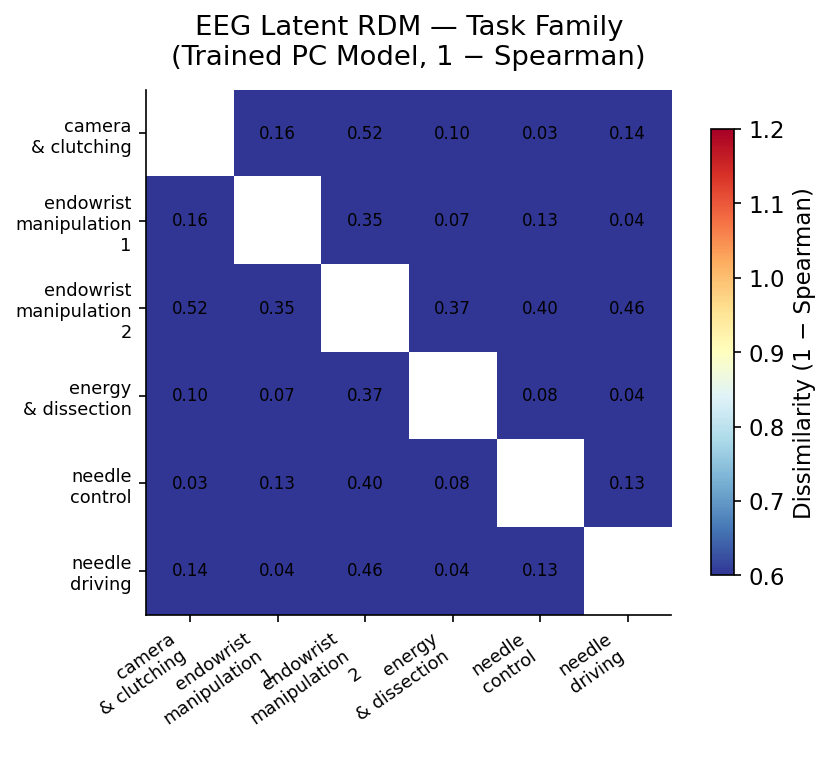
\includegraphics[width=0.72\textwidth]{fig3_eeg_latent_rdm.png}
  \caption{Representational Dissimilarity Matrix (RDM) from the trained PC model's
  latent state, grouped by surgical task family. Entries show pairwise dissimilarity
  ($1 - \text{Spearman}~r$). Diagonal entries (self-similarity) are masked. Warmer
  colors indicate greater dissimilarity. Needle control and camera-and-clutching tasks
  cluster together; energy-and-dissection tasks are most distinct.}
  \label{fig:rdm}
\end{figure}

\subsection{RDM Quality Comparison Across Representation Types}

Figure~\ref{fig:rdm_scores} and Table~\ref{tab:rdm_quality} compare quality scores
across all six candidate RDMs. The EEG latent RDM dominates on the interpretability
dimension ($0.81$) and ranks first in combined score ($0.32$). All eye-only and
joint RDMs score zero on interpretability, because the eye summary vectors produce
identical pairwise dissimilarities of $1.0$ between all task families---a degenerate
result that occurs when there is insufficient within-family variance to compute
Spearman correlation across the six conditions. The EEG latent RDM is consequently the
only representation recommended for potential downstream transfer.

\begin{figure}[H]
  \centering
  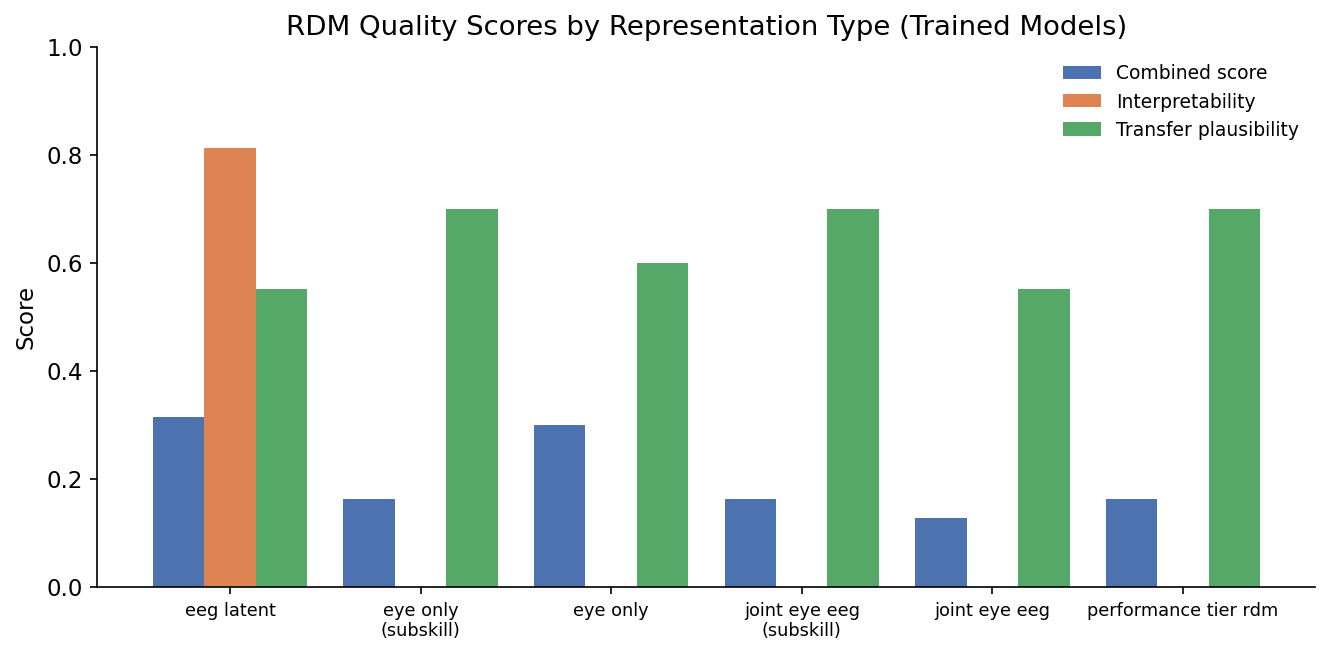
\includegraphics[width=0.95\textwidth]{fig4_rdm_scores.png}
  \caption{RDM quality scores across all six candidate representations. The EEG latent
  RDM is the only one with non-zero interpretability, reflecting that eye-only summaries
  collapsed to maximum pairwise dissimilarity under the current sampling strategy.}
  \label{fig:rdm_scores}
\end{figure}

\begin{table}[H]
\centering
\caption{RDM quality scores for trained models. Combined score is a weighted sum of
interpretability, eye-geometry agreement, and transfer plausibility.
$\checkmark$ denotes the representation recommended for downstream transfer.}
\label{tab:rdm_quality}
\begin{tabular}{lcccc}
\toprule
\textbf{RDM} & \textbf{Combined} & \textbf{Interpretability} & \textbf{Transfer} & \textbf{Rec.} \\
\midrule
EEG Latent (Task Family)         & 0.315 & 0.814 & 0.552 & $\checkmark$ \\
Eye Only (Task Family)           & 0.300 & 0.000 & 0.600 & \\
Eye Only (Subskill Family)       & 0.162 & 0.000 & 0.700 & \\
Joint Eye+EEG (Subskill Family)  & 0.162 & 0.000 & 0.700 & \\
Performance Tier                 & 0.162 & 0.000 & 0.700 & \\
Joint Eye+EEG (Task Family)      & 0.127 & 0.000 & 0.552 & \\
\bottomrule
\end{tabular}
\end{table}

% ══════════════════════════════════════════════════════════════════════════════
\section{Discussion}
% ══════════════════════════════════════════════════════════════════════════════

The central finding of this study is a training-induced dissociation between the latent
state and prediction error channels of a GRU-based predictive coding model. After
self-supervised training with a next-window prediction objective, the latent state $z_t$
became anti-correlated with eye-state occupancy, while the prediction error $\epsilon_t$
became positively correlated. This dissociation is not only statistically notable but
also theoretically coherent.

Under predictive coding theory, the latent state encodes the model's current
expectation of the sensory environment---the best guess about what is happening and
what will come next \citep{whittington2019theories}. A well-trained predictive model
should produce latent states that track the \textit{regular, predictable} aspects of
the input. Eye-state occupancy, by contrast, reflects the degree to which gaze is
allocated to fixation versus saccadic exploration---a signal driven partly by
unexpected or attention-demanding events. It is therefore conceptually consistent that
a trained latent state would \textit{not} align with eye occupancy: the latent state
tracks what is expected, while eye occupancy tracks what is novel or salient.

The prediction error, $\epsilon_t = e_t - \hat{e}_t$, captures precisely the
discrepancy between expected and observed EEG---the ``surprise'' signal. This is the
quantity that predictive coding theory identifies as the primary driver of
attention-related neural responses \citep{whittington2019theories}. That this signal
aligns with eye-state occupancy after training---achieving positive correlation in 59\%
of trials and a mean $r = +0.053$---supports the view that surprise-based EEG signals
track gaze allocation in a biologically meaningful way.

Interestingly, the baseline CNN shows more extreme anti-correlation than the PC latent
state after training ($r = -0.085$ vs. $r = -0.120$, but with near-zero variance). This
suggests the CNN learned a highly regular representation with almost no trial-to-trial
variability, consistent with a model that captured low-level temporal autocorrelation in
EEG without extracting cognitively meaningful structure. The PC model's latent state,
despite also becoming anti-correlated, retains substantially more trial-to-trial variance
(SD $= 0.074$ vs. SD $= 0.002$), suggesting richer encoding.

The EEG latent RDM is a further source of evidence that training produced meaningful
structure. The task-family geometry---with needle control and camera-and-clutching tasks
most similar, and energy-dissection tasks most distinct---maps loosely onto known
qualitative differences in motor demands across simulator tasks. This is encouraging
evidence that even a small, self-supervised model trained on 100 trials can learn some
degree of task-discriminating geometry from raw EEG.

One notable negative result is the failure of eye-only RDMs to produce interpretable
geometry. All eye-based RDMs yielded maximum pairwise dissimilarity between every pair
of task families, indicating that eye summary vectors collapsed to the same value across
conditions. This is likely a sampling artifact: with only one or a few trials per
task-family group, the Spearman correlation across the six conditions is undefined or
degenerate. This does not imply that eye tracking is uninformative---rather, it
suggests that the current aggregation strategy requires more trials per condition to
produce stable RDMs.

% ══════════════════════════════════════════════════════════════════════════════
\section{Limitations}
% ══════════════════════════════════════════════════════════════════════════════

Several limitations affect the strength of the conclusions drawn here.

\textbf{Model size and training data.} Both models are small (64-dimensional embeddings,
a 3-layer CNN and a single GRU cell) and trained on 100 trials. With 128 channels
$\times$ 500 time steps per window and an average of 264 windows per trial, the training
set provides substantial within-trial signal, but limited cross-trial diversity.
Representations trained on this scale may overfit to participant-specific or
session-specific EEG patterns and may not generalize.

\textbf{Random initialization as baseline.} The untrained results are based on random
model weights. While random-weight comparisons provide a useful reference for measuring
the effect of training, they do not constitute a comparison against a properly trained
baseline with a different objective. Future work should compare against a model trained
with contrastive or supervised objectives.

\textbf{Channel inconsistency.} EEG files in the dataset differed slightly in channel
count after MNE's automated EEG channel selection (126 or 128 channels). All models
were trained on the minimum channel count (126), and input windows were truncated
accordingly during inference. While this loses two channels of data for some trials,
the effect on results is expected to be negligible.

\textbf{Prediction error RDM unavailable.} The pipeline was unable to construct an RDM
from the prediction error representation due to shape inconsistencies across trials
(variable-length sequences). Future work should aggregate prediction errors to a fixed
summary vector per trial before constructing the RDM, which would allow direct
comparison of the prediction error's RDM geometry against the eye-only and latent RDMs.

\textbf{Fingerprint alignment not computed.} The fingerprint Spearman metric (which
compares the structure of individual trial representations across subjects) returned NaN
for all conditions, likely due to insufficient matched pairs. This metric could provide
a more fine-grained test of cross-participant consistency.

\textbf{Eye-only RDM degeneracy.} As discussed, the eye-only RDMs produced maximum
pairwise dissimilarity for all task-family pairs, making them uninformative as comparison
targets for the eye-geometry agreement metric. This limits our ability to evaluate
whether the EEG latent RDM geometry matches the eye-tracking geometry.

\textbf{No formal significance testing.} The analyses reported here are descriptive.
No permutation tests, confidence intervals, or corrections for multiple comparisons
were applied. Future work should include bootstrapped confidence intervals on the
occupancy Spearman values and permutation tests for the RDM correlations.

\textbf{Cross-dataset transfer not validated.} The project stops short of transferring
EEG-derived RDMs to the JIGSAWS surgical gesture dataset. Whether the representations
learned here carry useful geometry for ViT regularization in a different surgical domain
remains an open empirical question.

% ══════════════════════════════════════════════════════════════════════════════
\section{Methods}
% ══════════════════════════════════════════════════════════════════════════════

\subsection{Dataset}

We used the publicly available EEG and eye-gaze dataset for robot-assisted surgery
performance evaluation \citep{shafiei2023eeg}, which contains synchronized EEG and
eye-tracking recordings from 25 participants performing 27 tasks on a da Vinci surgical
simulator. EEG was recorded at 500~Hz with 128 active electrodes. Eye tracking was
recorded at 50~Hz capturing gaze position (x, y), pupil diameter (left and right), and
movement type classifications. Performance scores (0--100) are provided per trial.

For this study we used 100 trials sampled from the dataset (those with matching EEG and
eye files), spanning multiple participants and task types. Tasks were grouped into six
families: camera and clutching, endowrist manipulation I, endowrist manipulation II,
energy and dissection, needle control, and needle driving.

\subsection{EEG Preprocessing}

Raw EDF files were loaded using MNE-Python \citep{gramfort2013meg} with automatic EEG
channel selection (\texttt{pick\_types(eeg=True)}). All signals were bandpass filtered
between 1 and 40~Hz and notch filtered at 50~Hz to remove power-line noise. Filtered
EEG was segmented into overlapping 1-second windows with a 0.5-second hop
($n_{\text{time}} = 500$ samples per window). Across the 100 trials, an average of
264 windows were extracted per trial.

A small number of files yielded 126 channels after EEG channel selection (rather than
128), due to differences in electrode annotations across recording sessions. To ensure
consistent model input dimensions, all models were trained with $n_{\text{channels}} =
126$ (the minimum), and windows with 128 channels were truncated accordingly.

\subsection{Models}

\paragraph{Baseline CNN.}
The baseline encoder is a temporal convolutional network operating on single EEG windows
of shape $(n_{\text{channels}}, n_{\text{time}})$. It consists of three
\texttt{Conv1d} layers (channel sizes 64, 128, 128; kernel sizes 7, 5, 3) with ReLU
activations, followed by adaptive average pooling over the time dimension and a linear
projection to a 64-dimensional embedding. During training, a lightweight linear
prediction head ($\mathbb{R}^{64} \to \mathbb{R}^{n_{\text{channels}} \times
n_{\text{time}}}$) predicts the flattened next window, and this head is discarded after
training. Only the encoder weights are used for representation extraction.

\paragraph{Predictive Coding GRU.}
The PC model processes trial windows as a temporal sequence. Each window is flattened
and passed through a linear encoder ($\mathbb{R}^{n_{\text{channels}} \times
n_{\text{time}}} \to \mathbb{R}^{128}$) with ReLU activation. The resulting input
representation is fed into a single \texttt{GRUCell}, which maintains a 128-dimensional
hidden state $h_t$ that is updated recurrently as:
\begin{equation}
  h_t = \text{GRU}(\text{enc}(e_t),\; h_{t-1})
\end{equation}
A prediction head maps $h_t$ to a predicted next observation $\hat{e}_{t+1} \in
\mathbb{R}^{n_{\text{channels}} \times n_{\text{time}}}$, and the prediction error is:
\begin{equation}
  \epsilon_t = \left\| e_{t+1} - \hat{e}_{t+1} \right\|^2
\end{equation}
The latent embedding at each step is a linear projection of the hidden state:
$z_t = W_{\text{proj}}\, h_t \in \mathbb{R}^{64}$.

Three representations are extracted for analysis: (1) the per-window baseline CNN
embedding, (2) the per-window PC latent $z_t$, and (3) the per-window scalar prediction
error $\epsilon_t$.

\subsection{Self-Supervised Training}

Both models were trained with Adam (learning rate $10^{-3}$) for 20 epochs on the
100-trial dataset. The shared objective is next-window prediction via mean squared error.

For the baseline CNN, the loss at each step is:
\begin{equation}
  \mathcal{L}_{\text{baseline}} = \frac{1}{T-1}\sum_{t=1}^{T-1} \left\| W_{\text{pred}}\,\text{enc}(e_t) - \text{flat}(e_{t+1}) \right\|^2
\end{equation}
where $W_{\text{pred}}$ is the prediction head. The CNN processes all windows in a
single batched forward pass, enabling efficient training.

For the PC model, the loss is the mean per-step prediction error:
\begin{equation}
  \mathcal{L}_{\text{PC}} = \frac{1}{T-1}\sum_{t=1}^{T-1} \epsilon_t
\end{equation}
The GRU is trained using truncated backpropagation through time (TBPTT) with chunk
size 50 to keep memory bounded for long sequences. The hidden state is carried across
chunks but detached from the computational graph at each chunk boundary.

\subsection{Eye-Tracking Processing}

Eye-tracking CSVs were loaded and cleaned by removing noise epochs (movement type
codes 0 and 3) and interpolating blink-related zero-pupil periods. A Gaussian Hidden
Markov Model (HMM) with 3--5 states was fit to rolling window features (fixation ratio,
gaze dispersion, pupil standard deviation), inferring a state sequence over the trial.
When HMM fitting failed to converge, quantile-based binning was used as a fallback.
The output is an eye-state occupancy vector for each trial: the fraction of time spent
in each HMM state.

\subsection{Eye-Consistency Evaluation}

Eye-state occupancy alignment was measured by computing the Spearman correlation
between the trial-level EEG representation summary and the eye-state occupancy vector.
For each trial, the EEG representation summary was the mean over windows (for latent
embeddings) or the mean scalar value (for prediction errors). This yielded a single
Spearman $r$ per trial per representation type. We report mean, standard deviation,
and the fraction of trials with $r > 0$ across the 100 trials.

\subsection{Representational Dissimilarity Matrices}

Trial-level EEG summaries were grouped by task family (six groups). Within each group,
representations were averaged to yield a centroid vector. Pairwise dissimilarity between
groups was computed as $1 - r_s$, where $r_s$ is the Spearman correlation between the
two centroid vectors. This produced a $6 \times 6$ symmetric RDM with zero diagonal.

RDM quality was assessed along three axes: interpretability (off-diagonal variance,
reflecting how much structure the RDM encodes), eye-geometry agreement (Spearman
correlation between the EEG RDM and the eye-only task-family RDM), and transfer
plausibility (a prior score reflecting how well the task family maps onto the JIGSAWS
surgical domain). A combined score was computed as a weighted sum of these three metrics.

% ── references ────────────────────────────────────────────────────────────────
\newpage
\bibliographystyle{plainnat}
\bibliography{references}

\end{document}
